\documentclass{article}

% if you need to pass options to natbib, use, e.g.:
%     \PassOptionsToPackage{numbers, compress}{natbib}
% before loading neurips_2018

% ready for submission
% \usepackage{neurips_2018}

% to compile a preprint version, e.g., for submission to arXiv, add add the
% [preprint] option:
     \usepackage[final]{neurips_2018}

% to compile a camera-ready version, add the [final] option, e.g.:
%     \usepackage[final]{neurips_2018}

% to avoid loading the natbib package, add option nonatbib:
%     \usepackage[nonatbib]{neurips_2018}

\usepackage[utf8]{inputenc} % allow utf-8 input
\usepackage[T1]{fontenc}    % use 8-bit T1 fonts
\usepackage{hyperref}       % hyperlinks
\usepackage{url}            % simple URL typesetting
\usepackage{booktabs}       % professional-quality tables
\usepackage{amsfonts}       % blackboard math symbols
\usepackage{nicefrac}       % compact symbols for 1/2, etc.
\usepackage{microtype}      % microtypography
\usepackage{float}
\usepackage{graphicx}
\usepackage{amsmath,amssymb} 
\usepackage{physics}
\usepackage{longtable}
\usepackage{tabularx}
\usepackage{listings}
\usepackage{color}
\usepackage{subfig}
 
\definecolor{codegreen}{rgb}{0,0.6,0}
\definecolor{codegray}{rgb}{0.5,0.5,0.5}
\definecolor{codepurple}{rgb}{0.58,0,0.82}
\definecolor{backcolour}{rgb}{0.40,0.40,0.40}
 
\lstdefinestyle{mystyle}{
    %backgroundcolor=\color{backcolour},   
    commentstyle=\color{backcolour},
    keywordstyle=\color{codegreen},
    numberstyle=\tiny\color{codegray},
    stringstyle=\color{codepurple},
    basicstyle=\footnotesize,
    breakatwhitespace=false,         
    breaklines=true,                 
    captionpos=b,                    
    keepspaces=true,                 
    numbers=left,                    
    numbersep=5pt,                  
    showspaces=false,                
    showstringspaces=false,
    showtabs=false,                  
    tabsize=2
}



\lstset{style=mystyle}




\title{Deep Neural Networks - Jsneural}

% The \author macro works with any number of authors. There are two commands
% used to separate the names and addresses of multiple authors: \And and \AND.
%
% Using \And between authors leaves it to LaTeX to determine where to break the
% lines. Using \AND forces a line break at that point. So, if LaTeX puts 3 of 4
% authors names on the first line, and the last on the second line, try using
% \AND instead of \And before the third author name.

\author{%
  Jose Luis Silva\thanks{https://jseluis.github.io/} \\
  Department of Physics and Astronomy\\
  Uppsala University\\
  Uppsala, SE 751 20 \\
  \texttt{jose.silva@physics.uu.se} \\
  % Affiliation \\
  % Address \\
  % \texttt{email} \\
  % \AND
  % Coauthor \\
  % Affiliation \\
  % Address \\
  % \texttt{email} \\
  % \And
  % Coauthor \\
  % Affiliation \\
  % Address \\
  % \texttt{email} \\
  % \And
  % Coauthor \\
  % Affiliation \\
  % Address \\
  % \texttt{email} \\
}
\makeatletter
\renewcommand{\@noticestring}{}
\makeatother
\begin{document}
% \nipsfinalcopy is no longer used

\maketitle

\begin{abstract}
***** citations, references and more text to be updated very soon ************\\
In this report we will explore the implementation and deployment of a shallow and deep neural network for classification and, as part of the assignment, also provide details about applications in the MNIST dataset. In order to provide a better optimization experience (decrease the computational complexity by avoiding for loops and consequently speed-up the computations), the code uses methods from built-in libraries such as Numpy for vectorization and storage of common terms of the gradients between the layers during the backward propagation. The optimization was performed using the stochastic gradient-descent method along with mini-batches in order to handle large datasets. We used hot-encoding targets for the classification since K>2, softmax activation function for the last layer and cross-entropy loss function to estimate the cost function. JSneural network is very simple, fast and flexible, since you can create as many layer as needed by setting the number of nodes at each specific layer along with the activation functions which can be either sigmoid or ReLU. This is simply done by calling methods and attributes from the main JSneural class.

\end{abstract}

\section{Introduction}
In the last report, we solved a binary classification task to optimized parameters of a simple logistic regression model that can efficiently predict the probability mass function $p(y = 1 | x)$ of an event $y \in \{0,1\}$, given x on a specific interval $[0,1]$.  For a binary problem, we could have explored the one-hot encoding vector-valued output $y_i$, such that:
\begin{eqnarray}
\bf{y}_1&=&[1~0]^T \nonumber \\
\bf{y}_2&=&[0~1]^T
\end{eqnarray}
and the parameters of the model could be found by minimizing the likelihood represented by the cross-entropy loss function. In this report, we generalize our previous model for a full connected neural network through the linear combination of multiple layers. These layers can have different activation functions (ReLU or Sigmoid). In principle, we combine multiple nonlinear functions that describes an output variable y through different layers, where:
\begin{eqnarray}
y = f(x_1,..,x_p;\theta) + \epsilon
\end{eqnarray}
where $\epsilon$ is considered a stochastic noise, $\theta$ represents the parameters of the model and $\epsilon \approx N(0, \eta^2) \rightarrow 0$. For each input vector $\bold{x}_i $, we compute the following set of linear combinations:

\begin{eqnarray}
\bold{z} &=& \bold{x}  \bold{w} + b = 
\begin{bmatrix}
x_{11}^{(1)} & x_{12}^{(1)} &  \dots & x_{1K}^{(1)} \\ \\
x_{21}^{(1)} & x_{22}^{(1)} & \dots & x_{2K}^{(1)} \\
\vdots & \vdots & \dots & \vdots \\
x_{p1}^{(1)} & x_{p2}^{(1)} & \dots & x_{pK}^{(1)}
\end{bmatrix} ~\dot~
\begin{bmatrix}
w_{11}^{(1)} & w_{12}^{(1)} &  \dots & w_{1K}^{(1)} \\ \\
w_{21}^{(1)} & w_{22}^{(1)} & \dots & w_{2K}^{(1)} \\
\vdots & \vdots & \dots & \vdots \\
w_{p1}^{(1)} & w_{p2}^{(1)} & \dots & w_{pK}^{(1)}
\end{bmatrix}  + b \\
z_{i1}&=&\sum_{j=1}^{p} x_{ij} w_{j1} +b_{1}~~;~z_{i2}=\sum_{j=1}^{p} x_{ij} w_{j2} +b_{2} ~~ \dots ~~
z_{iK}=\sum_{j=1}^{p} x_{ij} w_{jK} +b_{K}
\end{eqnarray}
where i represents the input vectors, $p$ the number of features in each input vector, $b$ represents the  offset parameter and $\bold{w}$ the weights matrix. In our implementation, b is summed by broadcasting and the matrices have dimensions $x(N,p)$ and $w(p,K)$. This procedure allows the computation of the probability that each input vector $\bold{x}_i$ belongs to certain class k. For a shallow Neural Network, we compute the activation function of the previous linear combinations where the output for each node/class are expressed by the following equation:
\begin{eqnarray}
h_{ik}=\sigma(z_{ik})=\sigma(\sum_{j=1}^{p} x_{ij} w_{jk}+\beta_{k} ),~k=[1,..,K]
\end{eqnarray}
where k represents the class node with a particular hot-encoding target, K is the total number of classes (10 in MNIST dataset), i=[1,..,N] a specific input in the dataset and p (28x28 pixels for MNIST dataset) represents the total number of features. The probabilities related to each class are estimated through the softmax activation function ($\sigma$) over each $z_{ik}$: 
\begin{eqnarray}
h_{ik}&=&\sigma(z_{ik})=\frac{e^{z_{ik}}}{\sum_{l=1}^{K} e^{z_{il}}}
\label{softmax}
\end{eqnarray}
with the following set of recursive equations:
\begin{eqnarray}
h_{i1}&=&\sigma(\sum_{j=1}^{p} x_{ij} w_{j1}+\beta_{1} ) \nonumber \\
h_{i2}&=&\sigma(\sum_{j=1}^{p} x_{ij} w_{j2}+\beta_{1} ) \nonumber \\
&...& \nonumber \\
h_{iK}&=&\sigma(\sum_{j=1}^{p} x_{ij} w_{jK}+\beta_{K} )  \\
h^{(1)}&=&\begin{bmatrix}
h_{11}^{(1)} & h_{12}^{(1)} &  \dots & h_{1K}^{(1)} \\ \\
h_{21}^{(1)} & h_{22}^{(1)} & \dots & h_{2K}^{(1)} \\
\vdots & \vdots & \dots & \vdots \\
h_{p1}^{(1)} & h_{p2}^{(1)} & \dots & h_{pK}^{(1)}
\end{bmatrix} 
\label{two-layer}
\end{eqnarray}
where the matrix $\bold{h}$ represents the probability of a particular input $\bold{x}^T_i$ to be in a specific class k given an initial set of random bias and weights. For the MNIST case we have a total of 10 columns and 28x28 rows. Hence, the softmax regression maximum likelihood is used to estimate the cost function where the cross-entropy loss function is computed through the following equation:
\begin{eqnarray}
L_i= - \sum_{k=1}^{K}\hat{y}_{ik}\log (h_{ik})
\end{eqnarray}
with $\hat{y}_{ik}=1$ if $y_i = k$ and zero otherwise. This procedure is followed by an optimization of the model through the maximization of the likelihood for a given set of parameters. We use the cross-entropy loss $L_i$ for each input vector and take an average over the dataset to estimate the cost function $J$, where:
\begin{eqnarray}
J &=& -\frac{1}{n} \sum_{i=1}^{N} \sum_{k=1}^{K}\hat{y}_{ik}\log (h_{ik})
\end{eqnarray}

It is important to mention that the power of Neural Networks can be emphasized on the stacking of multiple layers as a generalization through the linear combination of the previous layers with different activation functions $\gamma$. The activation functions can increase the complexity of the Neural Network and each layer is responsible for mapping a hidden layer $\bf{h}^{(l-1)}$ into the next layer $\bf{h}^{(l)}$, such that:

\begin{eqnarray}
\bf{h}^{(l)} = \gamma(\bf{W}^{lT}\bf{h}^{(l-1)} + \bf{b}^{(l)T})
\label{rec}
\end{eqnarray}

which can be extended for L stacked layers, such that (\ref{rec}) can be rewritten as:
\begin{eqnarray}
\bf{h}^{(1)} &=& \sigma(\bf{W}^{(1)T}\bf{x} + \bf{b}^{(1)T}) \nonumber \\
\bf{h}^{(2)} &=& \sigma(\bf{W}^{(2)T}\bf{h}^{(1)} + \bf{b}^{(2)T}) \nonumber \\
\bf{h}^{(3)} &=& \sigma(\bf{W}^{(3)T}\bf{h}^{(2)} + \bf{b}^{(3)T}) \nonumber \\
&...& \nonumber \\
\bf{h}^{(L-1)} &=& \sigma(\bf{W}^{(L-1)T}\bf{h}^{(L-2)} + \bf{b}^{(L-2)T}) \nonumber \\
\bf{z}&=&\bf{W}^{(L)T}\bf{h}^{(L-1)} + \bf{b}^{(L)T} 
\end{eqnarray}

where $\sigma$ is the activation function. Hence, the softmax on the last layer for classification and in this particular assignment, we implemented the possibility of using either sigmoid or ReLU for the hidden layers, such as:
\begin{eqnarray}
\sigma(z_{ik}) &=& \left[1+\exp(-\sum_{j=1}^{p} x_{ij}w_{jk}  +b_k )\right]^{-1}\longrightarrow sigmoid \nonumber \\
\sigma(z_{ik}) &=& \{0,max(h_{ik})\} \longrightarrow ReLU 
\end{eqnarray}

We have used the mini-batches stochastic gradient descent method to reduce the complexity of the model, since if the number of inputs increases such as $n \rightarrow \infty$, the computational operations becomes very expensive. The main idea is to compute $\div_{\theta}J(\theta)$ for random batches of the dataset until the whole dataset is mapped. We have used this approximation for the MNIST dataset. The update of the parameters will be treated in the next session.

\section{Backpropagation in jsneural}

First, we consider a simple model where a single hidden layer is activated by a sigmoid function and multiple output units are activated through the softmax function. For one mini-batch $i$, we can compute the derivative of the cost with respect to each weight connecting the hidden units to the output unit. First let's consider the update of the weights $w_{ji}$ and offsets $b_i$ by using the chain rule with the binary cross-entropy loss function, such that:

\begin{eqnarray}
&&\frac{\partial{J}}{\partial{w_{ji}}} = \frac{\partial{J}}{\partial{z_{i}}} \frac{\partial{z_{i}}}{\partial{w_{ji}}}   =  \frac{\partial{J}}{\partial{z_i}} \left( \frac{\partial}{\partial{w_{ji}}}\right)\left(\sum_{j=1}^{p}h_{j}w_{ji}  + b_i\right) = \left(\frac{\partial{J}}{\partial{z_i}}\right) h_{j}
\nonumber \\
&&\frac{\partial{J}}{\partial{b_l}} = \frac{\partial{J}}{\partial{z_i}} \frac{\partial{z_i}}{\partial{b_l}}   =  \frac{\partial{J}}{\partial{z_i}} \left( \frac{\partial}{\partial{b_l}}\right)\left(\sum_{j=1}^{p}h_{j}w_{ji}  + b_i\right) = \left(\frac{\partial{J}}{\partial{z_i}}\right)\delta_{i,l}
\label{partial_cost}
\end{eqnarray}
From the equations (\ref{partial_cost}), we can estimate the partial derivative of the cross-entropy loss function with respect to $h_i$ :
\begin{eqnarray}
&&\frac{\partial{J}}{\partial{z_i}} =  \frac{1}{n}\sum_{i=1}^{n} \frac{\partial{L_i}}{\partial{z_i}}  = \frac{1}{n}\sum_{i=1}^{n} \frac{\partial{L_i}}{\partial{h_i}}\frac{\partial{h_i}}{\partial{z_i}} 
\label{costz}
\end{eqnarray}
such that:
\begin{eqnarray}
&&\frac{\partial{h_i}}{\partial{z_i}} = \left(\frac{\partial{}}{\partial{z_i}}\right)  \left[1+\exp(-\sum_{j=1}^{p}h_{j}w_{ji}  + b_i )\right]^{-1} = e^{-z_i}(1+e^{-z_i})^{-2} 
%%\\=
\end{eqnarray}
and since:
\begin{eqnarray}
h_i = (1+e^{-z_i}) ^{-1} \rightarrow e^{-z_i} = h^{-1} -1 = \frac{(1-h_i)}{h_i}
\end{eqnarray}
therefore the derivative of the sigmoid with respect to $z_i$ can be written as :

\begin{eqnarray}
&&\frac{\partial{h_i}}{\partial{z_i}} =  \frac{(1-p_i)(1+e^{-z_i})^{-2} }{p_i}=h_i(1-h_i)
\end{eqnarray}
The first partial derivative from equation (\ref{costz}) becomes:
\begin{eqnarray}
&&\frac{\partial{L_i}}{\partial{h_i}} =  -\frac{y_i}{h_i} + \frac{(1-y_i)}{(1-h_i)}
\end{eqnarray}
therefore:
\begin{eqnarray}
&&\frac{\partial{J}}{\partial{z_i}} =  \frac{1}{n}\sum_{i=1}^{n} \left[-\frac{y_i}{h_i} + \frac{(1-y_i)}{(1-h_i)} \right] \left[  \frac{(1-h_i)}{h_i} \right] = \frac{1}{n}\sum_{i=1}^{n} [ -y_i(1-h_i) + h_i(1-y_i)] \nonumber \\ &&=  \frac{1}{n}\sum_{i=1}^{n}(h_i-y_i)  \longrightarrow ~ \frac{\partial{J}}{\partial{w_{ji}}} = \frac{1}{n}\sum_{i=1}^{n}(h_i-y_i) h_j~~~~;~~~ \frac{\partial{J}}{\partial{b_{l}}} = \frac{1}{n}\sum_{i=1}^{n}(h_i-y_i)\delta_{i,l}
\end{eqnarray}
This is gradient of the cost with respect to the last layer, however, we need to use backpropagation for the lower layers. For a previous layer l=1, we have the weight $w^1_{kj}$ connecting input unit k to the hidden unit j (index for the hidden unit) with $h_j = [1+ \exp(-z^1_j)]^-1$. Therefore, the gradient can be written as :
\begin{eqnarray}
&&\frac{\partial{J}}{\partial{w_{kj}}} =  \frac{1}{n}\sum_{i=1}^{n} \frac{\partial{L_i}}{\partial{z^1_j}}\frac{\partial{z^1_j}}{\partial{w_{kj}}} =\frac{1}{n}\sum_{i=1}^{n} \frac{\partial{L_i}}{\partial{z_i}}\frac{\partial{z_i}}{\partial{h_j}}\frac{\partial{h_j}}{\partial{z^1_j}}\frac{\partial{z^1_j}}{\partial{w_{kj}}}
\label{der-cost-w}
\end{eqnarray}
And if we consider the softmax activation function for a classification with more than two classes on the output:
\begin{eqnarray}
h_{ik} = \frac{\exp(z_{ik})}{\sum_{c=1}^K \exp(z_{ic})}
\end{eqnarray}
with the cross-entropy loss function and derivatives defined as:
\begin{eqnarray}
L_i = -{\sum_{k=1}^K y_{ik}\log(h_{ik})} \longrightarrow \frac{\partial L_i}{\partial y_{ik}} = -\frac{y_{ik}}{h_{ik}}
\end{eqnarray}
Therefore, we can compute the following derivatives:
\begin{eqnarray}
\frac{\partial L_i}{\partial z_{il}} = \sum_{k=1}^K \frac{\partial L_i}{\partial h_{ik}}\frac{\partial h_{ik}}{\partial z_{il}} = \frac{\partial L_i}{\partial h_{ik}}\frac{\partial h_{ik}}{\partial z_{ik}} - \sum_{l \neq k} \frac{\partial L_i}{\partial h_{ik}}\frac{\partial h_{ik}}{\partial z_{il}} 
\label{deriv-cost-2}
\end{eqnarray}
since:
\begin{eqnarray}
\frac{\partial h_{ik}}{\partial z_{il}} = h_{ik}(\delta_{k,l} -h_{il})
\end{eqnarray}
Therefore:
\begin{eqnarray}
\frac{\partial L_i}{\partial z_{il}} = \frac{\partial L_i}{\partial h_{ik}}\frac{\partial h_{ik}}{\partial z_{ik}} - \sum_{l \neq k} \frac{\partial L_i}{\partial h_{ik}}\frac{\partial h_{ik}}{\partial z_{il}} = -y_{ik} (1-h_{ik}) - \sum_{l \neq k} y_{ik}h_{il} =  h_{ik}-y_{ik}
\label{deriv-cost}
\end{eqnarray}
In order to determine the corrections for the cost function with respect to the weights in the softmax layer (last layer) for a class K, we implemented the following expression:
\begin{eqnarray}
&&\frac{\partial{L}}{\partial{w_{ji}}} =  \sum_{i=1}^{n} \frac{\partial{L}}{\partial{z_i}}\frac{\partial{z_i}}{\partial{w_{ji}}}  = (h_i - y_i) h_j
\label{der0}
\end{eqnarray}
and therefore by considering K classes and the units in the hidden layer with index j, we can have the following expression:
\begin{eqnarray}
&&\frac{\partial{L}}{\partial{z^1_{j}}} =  \sum_{i=1}^{K} \frac{\partial{L}}{\partial{z_i}}\frac{\partial{z_i}}{\partial{h_{j}}} \frac{\partial{h_j}}{\partial{z^1_{j}}} = \sum_{i=1}^{K}  (h_{i}-y_{i})(w_{ji})(h_j (1-h_j))
\label{der1}
\end{eqnarray}
Combining equations (\ref{der1}) and (\ref{der-cost-w}) we can determine the corrections for the first layer as follows:
\begin{eqnarray}
&&\frac{\partial{L}}{\partial{w_{kj}}} = \frac{\partial{L}}{\partial{z^1_{j}}}\frac{\partial{z^1_j}}{\partial{w_{kj}}} =  \sum_{i=1}^{K} \frac{\partial{L}}{\partial{z_i}}\frac{\partial{z_i}}{\partial{h_{j}}} \frac{\partial{h_j}}{\partial{z^1_{j}}} \frac{\partial{z^1_j}}{\partial{w_{kj}}}= \sum_{i=1}^{K}  (h_{i}-y_{i})(w_{ji})(h_j (1-h_j))(x_k) \nonumber \\
\label{der2}
\end{eqnarray}
We implemented these set of equations for recursive iterations in order to compute the gradient of the error with respect to different activity neurons. Jsneural can compute the gradients for all weights in a network with any number of layers with two possible activation functions. The implementation is done by considering a matrix notation, where we store derivatives inside the objects (layers) of the class jsneural.  This memorization  speeds up the calculation of derivatives in different layers. We have used a pattern of the derivatives to propagate the error for L stacked layers. We used matrix formulation to compute the backpropagation with the following set of recursive formulas:

\begin{eqnarray}
&&\frac{\partial{J}}{\partial{W^L}} = \left[\frac{\partial{J}}{\partial{Z^L}}\sigma'(Z^{(L)})\right].H^{(L-1)}\\
&&\frac{\partial{J}}{\partial{W^{(L-1)}}} =\left[ \frac{\partial{J}}{\partial{Z^L}}\sigma'(Z^{(L)}) W^{L}\sigma'(Z^{(L-1)})\right]H^{(L-2)}\\
&&\frac{\partial{J}}{\partial{W^{(L-2)}}} =\left[ \frac{\partial{J}}{\partial{Z^L}}\sigma'(Z^{(L)}) W^{L}\sigma'(Z^{(L-1)}) W^{L-1}\sigma'(Z^{(L-2)})\right]H^{(L-3)}\\
&&\vdots \nonumber \\
&&\frac{\partial{J}}{\partial{W^{(0)}}} =\left[ \frac{\partial{J}}{\partial{Z^L}}\sigma'(Z^{(L)}) W^{L}\sigma'(Z^{(L-1)}) W^{L-1}\sigma'(Z^{(L-2)})\hdots W^1\sigma'(Z^{(0)}) \right] H^{(0)} \nonumber \\
\label{der2}
\end{eqnarray}

where $\sigma'(Z^L)$ represents the derivative of the activation function for a specific layer L, $H^{(L-1})$ represents the input from a previous layer which depends of the activation function from the previous layer (or softmax in case of only one layer for classification) and $W^L$ represents the weight matrix for the layer L. For each layer, the correction for the bias is estimated by considering only the operations inside the parenthesis without H.

The parameters of the model were updated through the following set of recursive formulas :
\begin{eqnarray}
W_l^L&:=&W_{(l-1)}^L -  \alpha \frac{\partial{J}}{\partial{W^L}}  \\
b_l^L&:=&b_{(l-1)}^L -  \alpha \frac{\partial{J}}{\partial{W^L}}\frac{1}{H^{(L-1)}}  \\
W_l^{(L-1)}&:=&W_{(l-1)}^{L-1} -  \alpha \frac{\partial{J}}{\partial{W^{(L-1)}}}  \\
b_l^{(L-1)}&:=&b_{(l-1)}^L -  \alpha \frac{\partial{J}}{\partial{W^{(L-1)}}} \frac{1}{H^{(L-2)}} \\ 
\vdots \nonumber \\
W_l^{(0)}&:=&W_{(l-1)}^{(0)} -  \alpha \frac{\partial{J}}{\partial{W^{(0)}}} \nonumber \\
b_l^{(0)}&:=&b_{(l-1)}^{(0)} -  \alpha \frac{\partial{J}}{\partial{W^{(0)}}} \frac{1}{H^{(0)}}  \nonumber \\
\end{eqnarray}

where l represents the iteration. In the next session we present the results from our implementation to predict handwritten numbers from MNIST dataset.

\section{Exercise 2.1}
\begin{figure}[!tbp]
  \centering
  \subfloat[Cost function x Iteration - Blue = Train data set , Red = Test data set]{\includegraphics[width=0.8\textwidth]{1a}\label{fig:f1}}
  \hfill
  \subfloat[Accuracy x Iteration - Blue = Train data set , Red = Test data set]{\includegraphics[width=0.8\textwidth]{1b}\label{fig:f2}}
  \caption{Convergence for Accuracy and Cost Function}
\end{figure}
For this assignment we have implemented the Softmax output using hot-encoding with 3 classes. I have replaced the sigmoid output from the last report in order to handle K > 2 classes. I have used the cross-entropy as loss function and mini-batch training. The first implementation replaces the gradient descent with mini-batch gradient descent to decrease the computational time during the training of larger datasets. I have used Python with Numpy library for vectorization and faster operations. In order to test the algorithm, I have created the following training dataset:  $n=8$ input vectors with two features $x_i=[x_1,x_2]$ and outputs that can be classified into 3 classes. Therefore, if $x_1=x_2$, $y_i = [1,0,0]$, for $x_2>x_1$ the output is $y_i = [0,1,0]$, otherwise, $y_i = [0,0,1]$. Hence, our training and test data sets are represented by the following arrays:
\begin{eqnarray}
&&X\_train = ([[1,1],[3,4],[5,5],[9,7],[6,4],[4,4],[10,1],[1,3]]) \\
&&Y\_train = ([[1,0,0],[0,1,0],[1,0,0],[0,0,1],[0,0,1],[1,0,0],[0,0,1],[0,1,0]])\\
&&X\_test = ([[3,3],[3,10],[1,5],[12,12],[2,2]])\\
&&Y\_test = ([[1,0,0],[0,1,0],[0,1,0],[1,0,0],[1,0,0]])\\
\end{eqnarray}
An initialization function was responsible for starting a set of parameter such as a fixed learning rate of 0.2 and break of the self-consistent loops based on values of the cost function based on the number of epochs. Since the mini-batch was implemented, we reshuffle the data set and recalculate the cost function and update the parameters of the model for every 4 inputs. The number of initial epochs was fixed to 10000 since the data set is very small. The set of equations for the softmax activation function was implemented along with the cost function and proper deduced gradients to update the parameters of the model for each mini-batch. The accuracy for the predictions on the training and test data set based on the optimized parameters was 100$\%$ as can be seen in the Figures \ref{fig:f1} and \ref{fig:f2}.The implementation is detailed in the appendix 1a. The noise of the cost function is related with the stochastic random cost functions generated by mini-batches that updates the parameters of the model for every iteration.

\begin{figure}[H]
  \centering
  \subfloat[Cost function x Iteration - Blue = Train data set , Red = Test data set]{\includegraphics[width=0.8\textwidth]{mnist1}\label{fig:mnist1}}
  \hfill
  \subfloat[Accuracy x Iteration - Blue = Train data set , Red = Test data set]{\includegraphics[width=0.8\textwidth]{mnist2}\label{fig:mnist2}}
  \caption{Convergence for Accuracy and Cost Function on MNIST dataset}
\end{figure}

%\begin{figure}[H]
%    \centering
%    \includegraphics[width=1\linewidth]{1a}
%    \caption{Cost function x Iteration - Blue = Test data set , Green = Train data set}
%    \label{fig:cancer}
%\end{figure}

We have applied the same optmization over the MNIST data, as can be seen in the implementation of the code in appendix 2a. For the MNIST dataset we have initialized the parameter with 0.8 for the learning rate, weight matrix generated randomly with Gaussian distributions where the standard deviation was fixed to 0.01. We have used the cross-entropy loss function to estimate the cost function and softmax activation with 10 output targets for classification of the handwritten dataset from 0 to 9. The mini-batch was fixed to 100 and after 10 epochs, the convergence showed high accuracy of 0.97131 on the training dataset and 0.97268 on the testing data set. For the training we reached the convergence after 10 epochs and 6000 iterations, as follows:

Epoch = 0 ; Cost Function = 1.6471016550976811 

Epoch = 1 ; Cost Function = 1.2243675446685733 

Epoch = 2 ; Cost Function = 1.0389976684215234 

Epoch = 3 ; Cost Function = 0.9054793401752557 

Epoch = 4 ; Cost Function = 0.8749678694293305 

Epoch = 5 ; Cost Function = 0.7862897065275499 

Epoch = 6 ; Cost Function = 0.685124613094569 

Epoch = 7 ; Cost Function = 0.6787356900239685 

Epoch = 8 ; Cost Function = 0.7620675345399908 

Epoch = 9 ; Cost Function = 0.6358987838271825 

Number of iterations =  6000

\begin{figure}[t]
     \centering
     \includegraphics[width=1\linewidth]{weight}
     \caption{Optimized weights (columns) after reshape (28x28 pixels)}
     \label{fig:figuree}
\end{figure}

As expected, the cost function and accuracy over both mini-batches and test data set decreases and increases with the number of iterations, respectively. We conclude with efficiently predicting the handwritten numbers from the MNIST test data set after 10 epochs. Additionally, the optimized parameters were reshaped to 28x28 pixels and plotted in Figure \ref{fig:figuree}. These images represents the weight filtering of the optimized model over the input data for further classification into one of the hot-encoding targets. 

\section{Exercise 2.2}

The previous code was generalized for any number of layers through the class jsneural, where we start with attributes that characterizes our neural network and methods to perform the optimization. The layers can be created with either ReLU or sigmoid activation functions by calling methods from the jsneural class. The last layer needs to be defined as softmax for proper classification. For each layer (object) we need to set the number of nodes and activation function. Therefore, the layer is an object inside jsneural class with attributes such as weight, bias, backpropagation term etc. which facilitates the operations for any number of layers using distinct activation functions. We have initialized the parameters of the model with learning rate of 0.3, batch size of 100 and 150 epochs. Our Neural network has 3 layers where the first layer is activated through the sigmoid function and the second layer is activated by ReLU. The first, second an third layers were defined with 100 nodes, 30 nodes and 10 nodes(classes from softmax), respectively. It's important to highlight that everything is automated and it is very easy to create any number of layers by setting the number of nodes and activation function commands. For this Neural Network we have 0.99006 accuracy over the MNIST test data. The cost for both training and test data is plotted along with iterations on the x-axis, as shown in Figure \ref{fig:mnist1a}. Additionally, Figure \ref{fig:mnist2b}  shows the classification accuracy evaluated on both test and training data. For the training data, we have evaluated both cost and accuracy over the current mini-batch during the iterations. The evaluation of  noise of the cost function and accuracy is mainly related with the stochastic characteristic of the optimization using mini-batches. The evolution of the accuracy and cost function within the iterations clearly shows the potential of this architecture to predict the testing handwritten numbers.


\begin{figure}[H]
  \centering
  \subfloat[Cost function x Iteration - Blue = Train mini-batch data set , Red = Test data set]{\includegraphics[width=0.8\textwidth]{mnist1-3layers}\label{fig:mnist1a}}
  \hfill
  \subfloat[Accuracy x Iteration - Blue = Train mini-batch data set , Red = Test data set]{\includegraphics[width=0.8\textwidth]{mnist2-3layers}\label{fig:mnist2b}}
  \caption{Accuracy and Cost Function on MNIST dataset using jsneural with 3 layers(Sigmoid, ReLU and Softmax)}
\end{figure}

\section{Future perspectives}

Our results have shown that jsneural implementation predicts the handwritten numbers from MNIST dataset with high accuracy and flexibility. As a perspective, I will extend the code with approaches such as Adam and RMSprop in order to control the optimization by modulating the learning rates, Convolutional Neural Networks and LSTM.


\newpage

\section{Appendix}
Exercise 2.1 
\begin{lstlisting}[language=Python]
# Import libraries
import numpy as np
import matplotlib.pyplot as plt
import pandas as pd
np.random.seed(1)

# The shape of x_train and x_test is (8, 3) and  y_test, y_train is (5,). Each vector has two features x1,x2 that belongs to one of 3 classes using the (hot encoding) [1,0,0][0,1,0] and [0,0,1] approximation. If x1=x2 [1,0,0], x1<x2 [0,1,0] and x1>x2 [0,0,1].

X_train = np.array([[1,1],[3,4],[5,5],[9,7],[6,4],[4,4],[10,1],[1,3]]) 
Y_train = np.array([[1,0,0],[0,1,0],[1,0,0],[0,0,1],[0,0,1],[1,0,0],[0,0,1],[0,1,0]])
X_test = np.array([[3,3],[3,10],[1,5],[12,12],[2,2]])
Y_test = np.array([[1,0,0],[0,1,0],[0,1,0],[1,0,0],[1,0,0]])

# Initialization of the parameters through initialize() function. The weights were chosen randomly using a normal distribution with gaussians with standard deviation of 0.01 and the initial offset was set to b = 0. loc = mean of the normal distribution, size = shape of the output, scale = standard deviation

def initialize(x_train,y_train):
    std_gaussian=0.01
    alpha = -0.2
    min_cost = 0.001
    epoch=10000
    batch_size=4
    counter = 0
    w = np.random.normal(size = ([x_train.shape[1],y_train.shape[1]]),loc=0,scale=std_gaussian) 
    n = x_train.shape[0]
    x = np.transpose(x_train)
    b = np.zeros([y_train.shape[1]])
    iterations=int(n/batch_size) # automated - based on the batch size
    return w,x,n,b,alpha,min_cost,epoch,batch_size,counter,iterations

# Definition of activation function sigma(z) based on the sigmoid. 
# Call the function sigma(z,activation='sigmoid'). 
def sigma(z_i,activation=False):
    if(activation==False):
        return print('Please choose an activation function')
    elif(activation=='sigmoid'):
        p_ik = 1/(1+np.exp(-z_i))
        return p_ik
    elif(activation=='softmax'):
        z_ik = np.exp(z_i)
        sum_row=np.sum(z_ik,axis=1).reshape(-1,1)
        p_ik=np.divide(z_ik,sum_row)
        return p_ik
    elif(activation=='relu'):
        p_ik = np.maximum(0.0,z_i)
        return p_ik

# This function calculates the cross-entropy loss function and the cost function. Instead of using for-loops element-wise operations are performed with arrays. Call the function : cost_function(y_train,p_i,loss_function='cross_entropy')

def cost_function(y_in,p_in,loss_function=False): 
    if(loss_function==False):
        return print('Please choose a loss function')
    elif(loss_function=='cross_entropy'):
        nb = y_in.shape[0]
        loss_calc = -np.sum(y_in*np.log(p_in),axis=1)
        cost_calc = (1/nb)*np.sum(loss_calc)
        return loss_calc,cost_calc
        
        
# This function calculates the gradients and performs matrix operations to estimate the partial derivatives. dLdb represents the derivative of the loss function with respect to the offset parameter b. dJdb = derivative of the cost function with respect to b and dJdw = derivative of the cost function with respect to a specific j-th weight. Numpy library was used for vectorization and to perform element-wise operations instead of for loops.  

def softmax_backward(p_in,y_in,x_in):
    n_in = y_in.shape[0]
    dLdb = p_in - y_in
    dJdb = (1/n_in)*np.sum(p_in-y_in,axis=0)
    dJdw = (1/n)*np.dot(np.transpose(x_in),dLdb) # vector dJ/dW_j to update w_j
    return dJdw,dJdb
    
# This function will randomly reshuffle X_train and Y_train with new indexes - mini-batches
def random_batch(x_in,y_in):
    random_index = np.random.choice(x_in.shape[0],size = x_in.shape[0], replace= False)
    x_out = x_in[random_index]
    y_out = y_in[random_index]
    return x_out,y_out

# Function to estimate the accuracy.
def accuracy(x_acc,y_acc,w,b):
    z_acc = np.dot(x_acc,w)+b
    p_ik_acc=sigma(z_acc,activation='softmax') # probability using optimized parameters
    p_ik_max_acc= np.max(p_ik_acc,axis=1).reshape(-1,1) # find maximum for each row and reshape to column
    y_pred_acc=np.where(p_ik_acc>=p_ik_max_acc,1,0) # change p_ik to 1 in case the element of the row is >= maximum for row.
    acc=np.mean(y_pred_acc == y_acc) # Calculate the accuracy
    return acc
    
# Initialize w=weight, x=input vectors, n= number of input vectors in the data set, alpha = learning rate, min_cost = control variable.
w,x,n,b,alpha,min_cost,epoch,batch_size,counter,iterations=initialize(X_train,Y_train)

# Main Loop using the mini-batches and epochs to optimize the parameter of the model
pred_acc=[] # array for accuracy prediction based on the iterations
pred_acc_test=[] # array for accuracy over the test dataset
cost = [] # array for cost function of mini-batch
cost_test = [] # array for cost function from test dataset
for E in range(epoch):
    X_train_minibatch,Y_train_minibatch = random_batch(X_train,Y_train) # reshuffle X_train and Y_train
    for i in range(iterations):
        x_loop = X_train_minibatch[i*batch_size:(i+1)*batch_size,:] # mini-batches
        y_loop = Y_train_minibatch[i*batch_size:(i+1)*batch_size,:] # mini-batches
        
        z = np.dot(x_loop,w)+b # feed-forward
        p_ik=sigma(z,activation='softmax') # softmax step to estimate probabilities
        l,j= cost_function(y_loop,p_ik,loss_function='cross_entropy') # cost function
        cost.append(j) # append cost of mini-batches        
        ztest = np.dot(X_test,w)+b # feed-forward with test dataset
        p_ik_test=sigma(ztest,activation='softmax') # calculate probability
        ltest,jtest= cost_function(Y_test,p_ik_test,loss_function='cross_entropy') # calculate cost for prediction
        cost_test.append(jtest) # append cost for test
        dw,db= softmax_backward(p_ik,y_loop,x_loop) # estimate correction for the bias and weight
        w +=alpha*dw # SGD to correct weight matrix
        b +=alpha*db # SGD to correct bias
        pred_acc.append(accuracy(x_loop,y_loop,w,b)) # calculate accuracy for x_loop
        pred_acc_test.append(accuracy(X_test,Y_test,w,b)) # append accuracy for test
        counter+=1
    print('Epoch =',E,'; Cost Function =',j,'\n')
print('Number of iterations = ',counter)

x=np.arange(1,counter+1) # generate x-axis for plotting

# Plot Cost function and Accuracy

plt.figure(dpi=120)
plt.plot(x,cost,c="b", marker="s", alpha=0.5,label="Cost minibatch")
plt.plot(x,cost_test,c="r", alpha=0.7,label="Cost test")
plt.xlabel("Iterations")
plt.ylabel("Cost Function ")
plt.legend(loc='upper right')
plt.figure(dpi=120)
plt.plot(x,pred_acc_test,c="r", marker="s", alpha=0.5,label="Accuracy - Test")
plt.plot(x,pred_acc,c="b", marker="s", alpha=0.5,label="Accuracy minibatch Train")
plt.xlabel("Iterations")
plt.ylabel("Accuracy")
plt.legend(loc='lower right')
plt.show()

# Accuracy 
accuracy(X_train,Y_train,w,b) # 100%
accuracy(X_test,Y_test,w,b) # 100%
\end{lstlisting}

Exercise 2.1 for MNIST dataset
\begin{lstlisting}[language=Python]
# Import libraries
import matplotlib.pyplot as plt
import numpy as np
import pandas as pd
from scipy import misc
import glob
import warnings
np.random.seed(1)
warnings.filterwarnings("ignore")
%matplotlib inline

# Import MNIST dataset and adjust data

def load_mnist():
    # Loads the MNIST dataset from png images
 
    NUM_LABELS = 10        
    # create list of image objects
    test_images = []
    test_labels = []    
    
    for label in range(NUM_LABELS):
        for image_path in glob.glob("MNIST/Test/" + str(label) + "/*.png"):
            image = misc.imread(image_path)
            test_images.append(image)
            letter = [0 for _ in range(0,NUM_LABELS)]    
            letter[label] = 1
            test_labels.append(letter)  
            
    # create list of image objects
    train_images = []
    train_labels = []    
    
    for label in range(NUM_LABELS):
        for image_path in glob.glob("MNIST/Train/" + str(label) + "/*.png"):
            image = misc.imread(image_path)
            train_images.append(image)
            letter = [0 for _ in range(0,NUM_LABELS)]    
            letter[label] = 1
            train_labels.append(letter)                  
            
    X_train= np.array(train_images).reshape(-1,784)/255.0
    Y_train= np.array(train_labels)
    X_test= np.array(test_images).reshape(-1,784)/255.0
    Y_test= np.array(test_labels)
    
    return X_train, Y_train, X_test, Y_test
    
 # load MNIST dataset 
 X_train, Y_train, X_test, Y_test = load_mnist()
 
 #reshape image 0
 x_train_image = X_train.reshape(X_train.shape[0],28,28)
 
 # Plot image X_train[0]
plt.imshow(x_train_image[0], cmap=plt.cm.binary)
print(Y_train[i])

# Initialization of the parameters through initialize() function. 

def initialize(x_train,y_train):
    std_gaussian=0.01
    alpha = -0.8
    epoch=10
    batch_size=100
    counter = 0
    w = np.random.normal(size = ([x_train.shape[1],y_train.shape[1]]),loc=0,scale=std_gaussian) 
    n = x_train.shape[0]
    x = np.transpose(x_train)
    b = np.zeros([y_train.shape[1]])
    iterations=int(n/batch_size) # automated - based on the batch size
    return w,x,n,b,alpha,min_cost,epoch,batch_size,counter,iterations

# Activation function
def sigma(z_i,activation=False):
    if(activation==False):
        return print('Please choose an activation function')
    elif(activation=='sigmoid'):
        p_ik = 1/(1+np.exp(-z_i))
        return p_ik
    elif(activation=='softmax'):
        z_ik = np.exp(z_i)
        sum_row=np.sum(z_ik,axis=1).reshape(-1,1)
        p_ik=np.divide(z_ik,sum_row)
        return p_ik
    elif(activation=='relu'):
        p_ik = np.maximum(0.0,z_i)
        return p_ik
        
# Estimate the cost function using cross-entropy loss function. You need to define which type of loss function to use: cost_function(y_train,p_i,loss_function='cross_entropy')
def cost_function(y_in,p_in,loss_function=False): # Calculate the loss and cost function using entering arrays
    if(loss_function==False):
        return print('Please choose a loss function')
    elif(loss_function=='cross_entropy'):
        nb = y_in.shape[0]
        loss_calc = -np.sum(y_in*np.log(p_in),axis=1)
        cost_calc = (1/nb)*np.sum(loss_calc)
        return loss_calc,cost_calc

# Softmax backward - backpropagation of the error to estimate the bias and weights
def softmax_backward(p_in,y_in,x_in):
    n_in = y_in.shape[0]
    dLdb = p_in - y_in
    dJdb = (1/n_in)*np.sum(p_in-y_in,axis=0)
    dJdw = (1/n)*np.dot(np.transpose(x_in),dLdb) # vector dJ/dW_j to update w_j
    return dJdw,dJdb
    
# This function will randomly reshuffle X_train and Y_train with new indexes for the 
def random_batch(x_in,y_in):
    random_index = np.random.choice(x_in.shape[0],size = x_in.shape[0], replace= False)
    x_out = x_in[random_index]
    y_out = y_in[random_index]
    return x_out,y_out

# Function to estimate accuracy   
def accuracy(x_acc,y_acc,w,b):
    z_acc = np.dot(x_acc,w)+b
    p_ik_acc=sigma(z_acc,activation='softmax') # probability using optimized parameters
    p_ik_max_acc= np.max(p_ik_acc,axis=1).reshape(-1,1) # find maximum for each row and reshape to column
    y_pred_acc=np.where(p_ik_acc>=p_ik_max_acc,1,0) # change p_ik to 1 in case the element of the row is >= maximum for row.
    acc=np.mean(y_pred_acc == y_acc) # Calculate the accuracy
    return acc
    
# Initialize w=weight, x=input vectors, n= number of input vectors 
# in the data set, alpha = learning rate, min_cost = control variable
w,x,n,b,alpha,min_cost,epoch,batch_size,counter,iterations=initialize(X_train,Y_train)

# Main loop for mini-batches. Comments on the previous (same code)
pred_acc=[]
pred_acc_test=[]
cost = []
cost_test = []
for E in range(epoch):
    X_train_minibatch,Y_train_minibatch = random_batch(X_train,Y_train)
    for i in range(iterations):
        x_loop = X_train_minibatch[i*batch_size:(i+1)*batch_size,:]
        y_loop = Y_train_minibatch[i*batch_size:(i+1)*batch_size,:]
            # print(y_loop,i) debug ok
        z = np.dot(x_loop,w)+b
            # print(z,i)      debug ok 
        p_ik=sigma(z,activation='softmax')
            # print(p_ik,i)   debug ok
        l,j= cost_function(y_loop,p_ik,loss_function='cross_entropy')
        cost.append(j)
        
        ztest = np.dot(X_test,w)+b
        p_ik_test=sigma(ztest,activation='softmax')
        ltest,jtest= cost_function(Y_test,p_ik_test,loss_function='cross_entropy')
        cost_test.append(jtest)
            # print(l,j,i)    debug ok
            # print('Cost Function =',j,'\n') debug ok
        dw,db= softmax_backward(p_ik,y_loop,x_loop)
            # print(dw,db,i)   debug ok
        w +=alpha*dw
        b +=alpha*db
        pred_acc.append(accuracy(x_loop,y_loop,w,b))
        pred_acc_test.append(accuracy(X_test,Y_test,w,b))
        counter+=1
    print('Epoch =',E,'; Cost Function =',j,'\n')
print('Number of iterations = ',counter)

x=np.arange(1,counter+1) # generate x-axis for plotting

# plot Cost and Accuracy 

plt.figure(dpi=120)
plt.plot(x,cost,c="b", marker="s", alpha=0.7,label="Cost minibatch")
plt.plot(x,cost_test,c="r", alpha=0.9,label="Cost test")
plt.xlabel("Iterations")
plt.ylabel("Cost Function ")
plt.legend(loc='upper right')
plt.figure(dpi=120)
plt.plot(x,pred_acc,c="b", marker="s", alpha=0.5,label="Accuracy minibatch Train")
plt.plot(x,pred_acc_test,c="r", marker="", alpha=0.8,label="Accuracy - Test")
plt.xlabel("Iterations")
plt.ylabel("Accuracy")
plt.legend(loc='lower right')
plt.show()

# Check accuracy over training and testing datasets

accuracy(X_train,Y_train,w,b)
accuracy(X_test,Y_test,w,b)

# Reshape the optimized weights
w_pictures = w.T.reshape(10,28,-1)

# Generate images of reshaped weights
for i in range(w_pictures.shape[0]):
    plt.imshow(w_pictures[i], cmap=plt.cm.binary)
    plt.show()
\end{lstlisting}

Exercise 2.2 for MNIST dataset
\begin{lstlisting}[language=Python]
# Import libraries
import numpy as np
import matplotlib.pyplot as plt
import pandas as pd
from scipy import misc
import glob
import warnings
np.random.seed(1)
warnings.filterwarnings("ignore")
%matplotlib inline

# Function for MNIST dataset
def load_mnist():
    # Loads the MNIST dataset from png images
 
    NUM_LABELS = 10        
    # create list of image objects
    test_images = []
    test_labels = []    
    
    for label in range(NUM_LABELS):
        for image_path in glob.glob("MNIST/Test/" + str(label) + "/*.png"):
            image = misc.imread(image_path)
            test_images.append(image)
            letter = [0 for _ in range(0,NUM_LABELS)]    
            letter[label] = 1
            test_labels.append(letter)  
            
    # create list of image objects
    train_images = []
    train_labels = []    
    
    for label in range(NUM_LABELS):
        for image_path in glob.glob("MNIST/Train/" + str(label) + "/*.png"):
            image = misc.imread(image_path)
            train_images.append(image)
            letter = [0 for _ in range(0,NUM_LABELS)]    
            letter[label] = 1
            train_labels.append(letter)                  
            
    X_train= np.array(train_images).reshape(-1,784)/255.0
    Y_train= np.array(train_labels)
    X_test= np.array(test_images).reshape(-1,784)/255.0
    Y_test= np.array(test_labels)
    
    return X_train, Y_train, X_test, Y_test
    
    # Load MNIST dataset into variables
    X_train, Y_train, X_test, Y_test = load_mnist()
    
# Function to initialize parameters inside the class jsneural
def initialize(x_train,y_train):
    jsneural.std_gaussian = 0.01 # standard deviation to generate the weights
    jsneural.alpha = -0.3 # learning rate
    jsneural.epoch = 5 # define the number of epochs
    jsneural.batch_size = 100 # define the batch size 
    jsneural.counter = 0 # counter inside the main loop
    jsneural.n = x_train.shape[0]  # number of inputs in the dataset
    jsneural.iterations=int(jsneural.n/jsneural.batch_size) # automated - based on the batch size
  
# Main class with initial attributes. The objects are the layers and the methods are called through jsneural.
  
class jsneural():
    Count = 0 
    alpha = [] 
    std_gaussian = []
    epoch = []
    batch_size = []
    n = []
    iterations = []
    counter = 0
    np.random.seed(10)
    layers = {} # dictionary used for internal loops - facilitate call of attributes from layers
    cost = [] # cost function
    cost_vector = [] # cost function array for plotting (mini-batches)
    cost_test_vector = [] cost function array for the test dataset
    acc_minibatch = []  # accuracy for the minibatch evaluated with iterations
    acc_test = [] # accuracy for the test evaluated with the iterations
    
    def __init__(self, input_x='False', output_y='False', n_nodes='False', activation='False'): # initalization of attributes
        self.x_train = input_x # input dataset X_train
        self.y_train = output_y # input dataset Y_train
        self.n_nodes = n_nodes # number of nodes of a specific layer
        self.activation = activation # activation function of a specific layer 
        self.w=[] # weight of a specific layer
        self.b=[] # bias of a specific layer
        self.dw=[] # correction for the weight for a specific laye r
        self.db=[] # correction for the bias for a specific layer
        self.H_term=[] # common term between layers for back-propagation
        self.z=[] # feed-forward for a specific layer
        self.h=[] # feed-forward with activation function for a specific layer
        self.h_derivative=[] # derivative of the activation function of a specific layer
        jsneural.layers.update({jsneural.Count:'layer'+str(jsneural.Count)}) # Create dictionary for each layer
        jsneural.Count += 1 # Counter add 1 every time a new object (layer) is defined
        
 ########## Start random parameters for the network ############

    def add_random(self,x):
        if (self.activation == "softmax"): # Generate matrix from previous layer (n_nodes)
            #self.w = np.random.normal(size = ([eval('layer'+str(jsneural.Count-2)+'.n_nodes'),self.y_train.shape[1]]),loc=0,scale=jsneural.std_gaussian) 
            self.w = np.random.normal(size = ([eval(jsneural.layers[x]+'.n_nodes')
                                               ,self.y_train.shape[1]]),loc=0,scale=jsneural.std_gaussian) 
            self.b = np.zeros([self.y_train.shape[1]])
        else:
            #self.w = np.random.normal(size = ([eval('layer'+str(x)+'.n_nodes'),self.n_nodes]),loc=0,scale=jsneural.std_gaussian) 
            self.w = np.random.normal(size = ([eval(jsneural.layers[x]+'.n_nodes')
                                               ,self.n_nodes]),loc=0,scale=jsneural.std_gaussian) 
            self.b = np.zeros([self.n_nodes])
  
    def generate_parameters(): # Loop to generate parameters for all the systems
        for i in range(jsneural.Count-1):
            eval(jsneural.layers[i+1]+'.add_random('+str(i)+')') # Run over dictionary
            #print(eval(jsneural.layers[i+1]+'.w')) debug ok
            #eval('layer'+str(i+1)+'.add_random('+str(i)+')') debug ok
            
 ##################################################

# Feed-forward for a specific layer
    def forward(self,x):
        self.z = np.dot(x,self.w)+self.b
        self.h = jsneural.sigma(self.z,activation=self.activation)
        self.h_derivative = jsneural.activation_derivatives(self,activation=self.activation)


# Derivative of activation function - sigmoid and ReLU
    def activation_derivatives(self,activation=False):
        if (self.activation == "sigmoid"):
            return self.h*(1-self.h) 
        elif (self.activation == "relu"):
            return np.where(np.maximum(0.0, self.h)>0,1,0)    
        else:
            return []

# Feed-forward for the whole model             
    def L_model_forward(x_minibatch):
        layer1.forward(x_minibatch)
        for i in range(jsneural.Count-2):
            eval('layer'+str(i+2)+'.forward(layer'+str(i+1)+'.h)')

# Update parameters of the model for each layer       
    def update_parameters(self,dw,db):
        self.w+=alpha*dw
        self.b+=alpha*db

# Check parameters of a specific layer    
    def parameters(self):
        weight = self.w
        bias = self.b
        return weight,bias
    
    ## Activation functions (ReLU, Sigmoid and Softmax)
    def sigma(z_i,activation=False):
        if(activation==False):
            return print('Please choose an activation function')
        elif(activation=='sigmoid'):
            p_ik = 1/(1+np.exp(-z_i))
            return p_ik
        elif(activation=='softmax'):
            z_ik = np.exp(z_i)
            sum_row=np.sum(z_ik,axis=1).reshape(-1,1)
            p_ik=np.divide(z_ik,sum_row)
            return p_ik
        elif(activation=='relu'):
            p_ik = np.maximum(0.0,z_i)
            return p_ik

# Compute the cost function for a specific layer       
    def compute_cost(y_in,loss_function=False): # Calculate the loss and cost function using entering arrays
        if(loss_function==False):
            return print('Please choose a loss function')
        elif(loss_function=='cross_entropy'):
            h_in = eval(jsneural.layers[jsneural.Count-1]+'.h')
            nb = y_in.shape[0]
            loss_calc = -np.sum(y_in*np.log(h_in),axis=1)
            jsneural.cost = (1/nb)*np.sum(loss_calc)
            return jsneural.cost

# First back-propagation from the softmax(last layer) layer.    
    def softmax_backward(self,p_in,x_in,y_in):
        n_in = y_in.shape[0]
        self.H_term = p_in - y_in
        self.db = (1/n_in)*np.sum(self.H_term,axis=0)
        self.dw = (1/n_in)*np.dot(np.transpose(x_in),self.H_term) # vector dJ/dW_j to update w_j for softmax

# Back-propagation for the other layers    
    def linear_backward(self,j,n_in):
        #print(' activation =',self.activation,'; layer =',j) #debugged - passed attributes
        H_next_layer = eval(jsneural.layers[j+1]+'.H_term')
        w_next_layer = eval(jsneural.layers[j+1]+'.w')
        H_previous_layer = eval(jsneural.layers[j-1]+'.h')
        HwT = np.dot(H_next_layer,w_next_layer.T)
        self.H_term = np.multiply(self.h_derivative,HwT) # memorization of commom term to backpropagate
        self.db = (1/n_in)*np.sum(self.H_term,axis=0)
        self.dw = (1/n_in)*np.matmul(H_previous_layer.T,self.H_term)

# Back-propagation for all layers in the model    
    def L_model_backward(x_back,y_back):     
        layer0.h = x_back
        n_in = y_back.shape[0]
        h_L=eval(jsneural.layers[jsneural.Count-1]+'.h')
        h_L_previous=eval(jsneural.layers[jsneural.Count-2]+'.h')
        eval(jsneural.layers[jsneural.Count-1]+'.softmax_backward(h_L,h_L_previous,y_back)')
        
        for i in range(jsneural.Count-2,0,-1): # Generalization for all layers - ok
            eval(jsneural.layers[i]+'.linear_backward(i,n_in)') #

# update parameters of each class    
    def update_parameters(self):
        self.w += jsneural.alpha*self.dw
        self.b += jsneural.alpha*self.db
        
# loop to update parameters 
    def L_model_update_parameters():
        for k in range(jsneural.Count-1,0,-1):
            eval(jsneural.layers[k]+'.update_parameters()')
            
# Reshuffle dataset for mini-batches
    def random_mini_batches(x_in,y_in):
        random_index = np.random.choice(x_in.shape[0],size = x_in.shape[0], replace= False)
        x_out = x_in[random_index]
        y_out = y_in[random_index]
        return x_out,y_out

# main method to train the neural network. The loss-function needs to be called.
    def train_L_layer_model(X_train,Y_train,loss_function=False):
        jsneural.counter=0
        for E in range(jsneural.epoch):
            X_train_minibatch,Y_train_minibatch = jsneural.random_mini_batches(X_train,Y_train)
            for i in range(jsneural.iterations):     
                x_loop = X_train_minibatch[i*jsneural.batch_size:(i+1)*jsneural.batch_size,:]
                y_loop = Y_train_minibatch[i*jsneural.batch_size:(i+1)*jsneural.batch_size,:]
                
                jsneural.L_model_forward(X_test)
                jsneural.compute_cost(Y_test,loss_function) # update jsneural.cost with test data
                jsneural.cost_test_vector.append(jsneural.cost)
                
                acc=jsneural.accuracy(Y_test)
                jsneural.acc_test.append(acc)
                
                jsneural.L_model_forward(x_loop)
                jsneural.compute_cost(y_loop,loss_function) # update jsneural.cost with mini-batch
                jsneural.cost_vector.append(jsneural.cost)
                
                acc=jsneural.accuracy(y_loop)
                jsneural.acc_minibatch.append(acc)
                
                jsneural.L_model_backward(x_loop,y_loop)
                jsneural.L_model_update_parameters()
                
                jsneural.counter+=1
            print('Epoch =',E,'; Cost Function =',jsneural.cost,'\n')
        print('Number of iterations = ',jsneural.counter)

# Estimate accuracy        
    def accuracy(yy):
        h = eval('layer'+str(jsneural.Count-1)+'.h')
        h_max_acc = np.max(h,axis=1).reshape(-1,1)
        y_pred=np.where(h>=h_max_acc,1,0)
        acc = np.mean(y_pred == yy)
        return acc

# Update a layer with a different number of nodes
    def update_layer(self, input_x='False', output_y='False', n_nodes='False', activation='False'):
        self.x_train = input_x
        self.y_train = output_y
        self.n_nodes = n_nodes
        self.activation = activation
        self.w=[]
        self.b=[]
        self.z=[]
        self.h=[]
        jsneural.layers.update({jsneural.Count:'layer'+str(jsneural.Count)}) # Create dictionary for each layer
        jsneural.Count = jsneural.Count

# initialize parameters of the model
initialize(X_train,Y_train)

# Create the object layer 0 with 28x28 nodes (number of features)
layer0 = jsneural(input_x=X_train,n_nodes=784) 

# Create the layer 1 with 100 nodes and sigmoid activation function
layer1 = jsneural(n_nodes=100,activation="sigmoid")

# Create layer2 with 30 nodes and ReLU activation function
layer2 = jsneural(n_nodes=30,activation="relu")

# Create the last layer with softmax for classification (automated)
layer3 = jsneural(output_y=Y_train,activation="softmax") 

# Generate the parameters of the model randomly with Gaussian distributions and stardard deviation of 0.01, bias = 0.
jsneural.generate_parameters()

# Train the NN
jsneural.train_L_layer_model(X_train,Y_train,loss_function='cross_entropy') 

x=np.linspace(1,jsneural.counter,jsneural.counter)

# Plot of accuracy and cost function for mini-batches and testing dataset.
plt.figure(dpi=120)
plt.plot(x,jsneural.cost_vector,c="b", alpha=0.7,label="Cost minibatch")
plt.plot(x,jsneural.cost_test_vector,c="r", alpha=0.7,label="Cost test")
plt.xlabel("Iterations")
plt.ylabel("Cost Function ")
plt.legend(loc='upper right')
plt.figure(dpi=120)
plt.plot(x,jsneural.acc_minibatch,c="b",alpha=0.7,label="Accuracy minibatch Train")
plt.plot(x,jsneural.acc_test,c="r", alpha=0.7,label="Accuracy - Test")
plt.xlabel("Iterations")
plt.ylabel("Accuracy")
plt.legend(loc='lower right')
plt.show()

# definition of a function for feed-forward outside of the class.
def prediction_forward(xx,yy):
    z = np.dot(xx,layer1.w)+layer1.b
    h = jsneural.sigma(z,activation=layer1.activation)
    for k in range(jsneural.Count-2):
        w_layer = eval('layer'+str(k+2)+'.w')
        b_layer = eval('layer'+str(k+2)+'.b')
        act = eval('layer'+str(k+2)+'.activation')
        z = np.dot(h,w_layer)+b_layer
        h = jsneural.sigma(z,activation=act)
    h_max_acc = np.max(h,axis=1).reshape(-1,1)
    y_pred=np.where(h>=h_max_acc,1,0)
    acc = np.mean(y_pred == yy)
    return acc,y_pred
    
# Feed-forward with the test dataset
accuracy,y_pred=prediction_forward(X_test,Y_test) 
print(accuracy) # 0.99006
\end{lstlisting} 

\section{References}
***** citations, references and more text to be updated ************
\end{document}
